% !TEX root = ../Coherence.tex

\begin{figure}
\centering
  \resizebox{4cm}{!}{
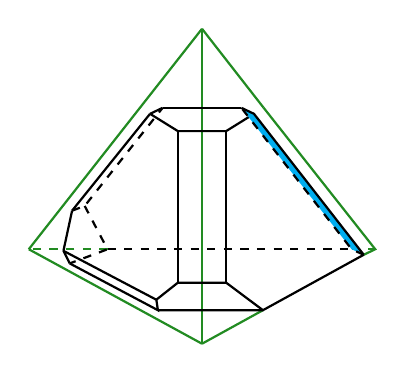
\begin{tikzpicture}[thick,scale=2]
\coordinate (A1) at (0,2);
\coordinate (A11) at (-0.39,1.5);
\coordinate (A111) at (-0.25,1.498);
\coordinate (A112) at (-0.33,1.46);
\coordinate (A12) at (0.39,1.5);
\coordinate (A121) at (0.25,1.498);
\coordinate (A122) at (0.33,1.46);
\coordinate (A13) at (0,1.25);
\coordinate (A131) at (-0.153,1.35); 
\coordinate (A132) at (0.153,1.35); 
\coordinate (A2) at (0,0); 
\coordinate (A21) at (-0.387,0.213); 
\coordinate (A211) at (-0.29,0.2795); 
\coordinate (A212) at (-0.28,0.213); 
\coordinate (A22) at (0.387,0.213); 
\coordinate (A23) at (0,0.5); 
\coordinate (A231) at (-0.153,0.388); 
\coordinate (A232) at (0.153,0.388); 
\coordinate (A3) at (-1.1,0.6);
\coordinate (A31) at (-0.9,0.49);
\coordinate (A311) at (-0.88,0.59);
\coordinate (A312) at (-0.84,0.51);
\coordinate (A32) at (-0.8,0.976);
\coordinate (A321) at (-0.825,0.845);
\coordinate (A322) at (-0.745,0.875);
\coordinate (A33) at (-0.6,0.6);
\coordinate (A4) at (1.1,0.6);
\coordinate (A41) at (1.027,0.565);
\coordinate (A42) at (0.95,0.6);
%\draw[draw=none,fill=cyan!40,opacity=0.5] (A42)--(A41)--(A121)--(A122)-- cycle;
\draw[draw=ForestGreen]  (A3)--(A2);
\draw[draw=ForestGreen]  (A1)--(A12);
\draw[draw=ForestGreen] (A2)--(A22);
\draw[draw=ForestGreen] (A2) -- (A1);
\draw[draw=ForestGreen] (A3)--(A1);
\draw[draw=ForestGreen,dashed]  (A33) -- (A3);
\draw[draw=ForestGreen,dashed]  (A42) -- (A4);
\draw[draw=ForestGreen] (A41)--(A4)--(A12);
 \draw[draw=black,fill=none]   (A321)--(A311);
 \draw[draw=black,fill=none] (A212)-- (A22) -- (A41);
\draw (A311)--(A312);
\draw (A111)--(A121);
\draw (A111)--(A112);
\draw (A311)--(A211)--(A212) --(A312);
\draw (A112)--(A321);
\draw[dashed] (A321)--(A322)--(A111);
\draw  (A211)--(A231)--(A232)--(A22);
\draw[dashed]  (A33) -- (A42);
\draw (A231) -- (A131) -- (A132) -- (A232) -- cycle;
\draw[dashed] (A322) -- (A33) -- (A312);
\draw (A112) -- (A131) --(A132)--(A122);
\fill[cyan] (A41) -- (A42) -- (A121)--(A122)--cycle;
\draw[dashed]  (A41) -- (A42) -- (A121); 
\draw (A41)--(A122) --(A121);
\end{tikzpicture}} \quad\quad  
\raisebox{1em}{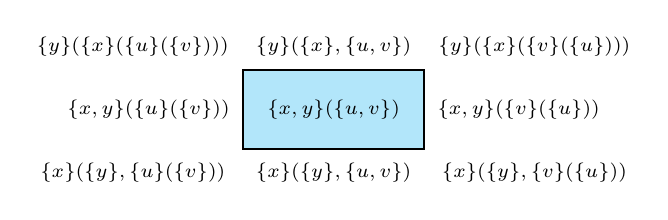
\begin{tikzpicture}[thick]
\coordinate (S1) at (-0.15,0);
\coordinate (S2) at (2.15,0);
\coordinate (S3) at (2.15,1);
\coordinate (S4) at (-0.15,1);
\draw[fill=cyan,opacity=0.3] (S1)--(S2)--(S3)--(S4)-- cycle;
\draw (S1)--(S2)--(S3)--(S4)-- cycle;
\node (s1) at (-1.55,-0.3) {\scriptsize $\{x\}(\{y\},\{u\}(\{v\}))$};
\node (s2) at (3.55,-0.3) {\scriptsize $\{x\}(\{y\},\{v\}(\{u\}))$};
\node (s4) at (-1.55,1.3) {\scriptsize $\{y\}(\{x\}(\{u\}(\{v\})))$};
\node (s3) at (3.55,1.3) {\scriptsize $\{y\}(\{x\}(\{v\}(\{u\})))$};
\node (s14) at (-1.35,0.5) {\scriptsize $\{x,y\}(\{u\}(\{v\}))$};
\node (s23) at (3.35,0.5) {\scriptsize $\{x,y\}(\{v\}(\{u\}))$};
\node (s12) at (1,-0.3) {\scriptsize $\{x\}(\{y\},\{u,v\})$};
\node (s34) at (1,1.3) {\scriptsize $\{y\}(\{x\},\{u,v\})$};
\node (s) at (1,0.5) {\scriptsize $\{x,y\}(\{u,v\})$};

\end{tikzpicture}}
\caption{A truncated simplex. \label{hemiassoc}}
\end{figure}